\setcounter{chapter}{1}
\setcounter{section}{0}
%\chapter{Introduction}
\setlength{\headheight}{12.71342pt}
\addtolength{\topmargin}{-0.71342pt}

\section{Introduction}
Fruits are complex and heterogeneous structures that comprise  a wide variety of metabolites that serve as precursors to volatile organic compounds (VOCs), such as carbohydrates, fatty acids, and pigments \cite*{A03_PanoFarias2017}. The mango fruit is no exception of this complexity and have in recent years been the focus of many studies, studying the activity of volatiles in the fruit \cite*{A04_GUO2023112779}.

\subsection{Background}
Mango is a tropical fruit which belongs to the Anacardiaceae family and is scientifically known as \textit{Mangifera} \cite*{A04_GUO2023112779}. It is popularly characterised as a sweet, juicy, aromatic fruit with a low fibre flesh \cite*{A05_Chin2019}. It is primarily cultivated in tropical and subtropical regions, where it is of significant economic importance \cite*{A05_Chin2019}. 
The annual tropical production of mango is over 46 million tons and is thereby the most produced tropical fruit after banana \cite*{A07_Bonneau2016}. The perishable nature and susceptibility to post-harvest losses and diseases pose challenges for the mango industry, restricting the production and potential \cite*{A05_Chin2019}.

\subsection{Focus on Mango}
The mango is an important fruit crop worldwide, valued for its high nutritional content, with significant levels of fibre, vitamin C and $\beta$-carotene \cite*{A01_Aguirre-Lopez_2023, A07_Bonneau2016}. However, beyond its nutritional benefits, the mango is particularly renowned for its distinctive aroma, which plays a crucial role in consumer preference and marketability \cite*{A06_Badar2016}. s of quality and freshness \cite*{A05_Chin2019}.
A study by Badar et al. (2016) found that aroma is one of the most important quality attributes that influence consumer preference and acceptance of mango fruit \cite*{A06_Badar2016}. The main aroma contributors in mango are the VOCs; aldehydes, alcohols, esters and ketones \cite*{A02_Moreno2010}. Among these, 3-carene, limonene, $\beta$-pinene, acetaldehyde, ethanol and hexanal \cite*{A02_Moreno2010}. Understanding the origin and behaviour of these volatiles is therefore essential for improving fruit quality, post-harvest handling, and processing applications.

\subsection{Aim and Scope}
The aim of this report is to explore the formation, composition, and significance of VOCs in mango fruits. The main focus is on how these compounds contribute to the fruit's aroma and overall quality, both in terms of maintaining freshness and enhancing consumer appeal.
The scope includes an overview of the chemical classes and key VOCs identified in mango, the metabolic- and enzymatic pathways involved in their biosynthesis, and the influence of pre- and post-harvest conditions on their abundance. Finally, the report outlines the methods commonly applied for the extraction and identification of VOCs and their relevance for assessing fruit quality and consumer perception.


\section{Aroma Composition in Mango}
The complexity of aromas in mango is due to the variety of VOCs that are present in the fruit's matrix. These compounds arise from different biochemical pathways and contribute to the overall sensory experience of the fruit \cite*{A05_Chin2019}. These pathways are most prominently manifested during the ripening processes of the fruit. Also visual and textural changes occur during ripening, which further influence the perception of aroma \cite*{A01_Aguirre-Lopez_2023, A05_Chin2019}.

\subsection{Chemical Classes of Mango Aroma Compounds}
The volatile composition in fresh mango fruits has been extensively studied, revealing a diverse array with several hundred identified volatile compounds, occuring in free form in the fruit \cite*{A07_Bonneau2016}. By calculating the flavour dilution factor (FD) of the volatile compounds using gas chromatography-olfactometry (GC-O) analysis, it has been possible to identify the key aroma compounds for the odour-active fraction \cite*{A07_Bonneau2016}.

Mango aroma is primarily composed of several chemical classes. The most dominant classes is monoterpene hydrocarbons, which account for 90.2\% of the total volatile compounds in fresh mango, as illustrated in Figure \ref{fig:mango_aroma_compounds}. Other significant classes include lactones (4.1\%) and sesquiterpene hydrocarbons (3.0\%) \cite*{A07_Bonneau2016}. 

\begin{figure}
    \centering
    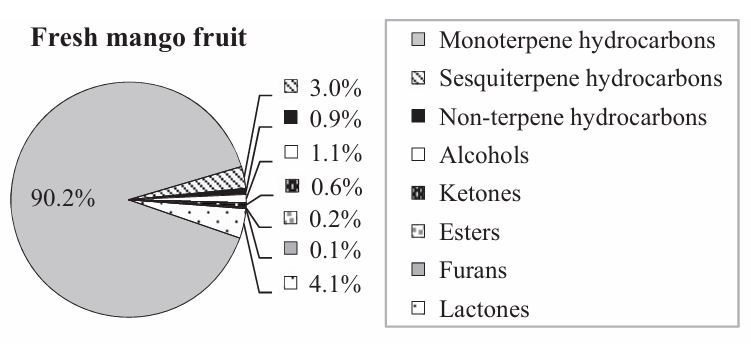
\includegraphics[width=0.8\textwidth]{Figures/fig_fresh_mango_chemical_classes.JPG}
    \caption{Distribution $[\%]$ of chemical classes of volatile compounds in fresh mango. Adapted from Bonneau et al. (2016) \cite*{A07_Bonneau2016}.}
    \label{fig:mango_aroma_compounds}
\end{figure}

\subsection{Key Aroma Compounds in Mango}
In this subsection, the key aroma compounds identified from fresh mango fruits in the study by Bonneau et al. (2016) are discussed \cite*{A07_Bonneau2016}. .

\subsubsection*{Terpenes and Terpenoids}
Terpenes represent the largest class of mango aroma compounds, derived from isoprene units via the terpenoid biosynthetic pathway \cite*{A09_Barras2024}. They include both monoterpenes and sesquiterpenes, which together account for the majority of mango volatiles \cite*{A07_Bonneau2016}. Terpenes and terpenoids are found in many different natural sources, including fruits, plants, animals, microbes, and fungi. The terpenes belong to the largest class of secondary metabolites in nature and consist of five connected carbon atoms, known as isoprene units. These carbon units can be assembled in thousands of ways \cite*{B01_TerpenesTerpenoids_2018}. The terpenoids are further subcualified into five sub-groups based on the number of isoprene units they contain: monoterpenes (C10), sesquiterpenes (C15), diterpenes (C20), sesterterpenes (C25), and triterpenes (C30) \cite*{B01_TerpenesTerpenoids_2018}.


\paragraph*{Monoterpene hydrocarbons}
A total of 11 monoterpene hydrocarbons were identified as key aroma compounds in fresh mango \cite*{A07_Bonneau2016}. The most significant ones include: $\alpha$-phellandrene, $\gamma$-terpinene, $\delta$-3-carnene, $\beta$-myrcene, $\alpha$-terpinene, limonene, $\beta$-phellandrene, and $\alpha$-terpineol. 

Monoterpenes are the smallest molecules in the isoprenoid family with conserved hydrocarbons \cite*{A09_Barras2024}. They share the formula $C_{10}H_{16}$ and over 400 different chemical structures has been classified as such \cite*{A09_Barras2024}. The key monoterpene hydrocarbons identified in mangos are reported to have significant impact on the overall odorants \cite*{A07_Bonneau2016}.

\paragraph*{Sesquiterpene hydrocarbons}
Compared to monoterpenes, sesquiterpenes are larger molecules with the formula $C_{15}H_{24}$. In mango fruit, the study by Bonneau et al. (2016) identified four key sesquiterpene hydrocarbons, including: $\alpha$-gurjunene, $\alpha$-copaene, $\beta$-caryophyllene, and $\alpha$-caryophyllene \cite*{A07_Bonneau2016}.

\subsubsection*{Alcohols and Aromatic Alcohols}
Alcohols and aromatic alcohols are, like terpenes and terpenoids, major contributors to the key aroma of mango, though they differ in chemical structure and biosynthetic origin. A study by Singh et al. (2010) highlighted the role of alcohol dehydrogenase (ADH) in the enzymatic reduction of aldehydes leading to the formation of these compounds \cite*{A10_Singh2010}.

\vspace{0.5em}
A total of nine alcohols were identified as key aroma compounds in fresh mango \cite*{A07_Bonneau2016}. The most significant ones include: 2-methyl-1-propanol, 1-pentanol, (\textit{E})-2-penten-1-ol, (\textit{Z})-2-penten-1-ol, 1-octanol, 1-butanol, 3-methyl-1-butanol, 2-decanol, 1-hexanol, and (\textit{Z})-3-hexen-1-ol \cite*{A07_Bonneau2016}.

\subsubsection*{Aldehydes and Aromatic Aldehydes}
Aldehydes are volatile compounds primarily formed through the oxidation of unsaturated fatty acids, such as $\alpha$-linolenic acid, via the lipoxygenase (LOX)–hydroperoxide lyase (HPL) pathway. These reactions generate C$_6$ and C$_9$ aldehydes, often referred to as green leaf volatiles, which are associated with fresh and grassy notes in the mango fruit aroma \cite*{A11_Sivankalyani2017}. In mango, this pathway becomes particularly active under chilling stress, leading to increased levels of compounds such as \textit{1-hexanal}, \textit{(E)-2-hexenal}, and \textit{(Z)-3-hexenal} before visible quality loss occurs.

In fresh mango, a total of six aldehydes were identified as key aroma compounds \cite*{A07_Bonneau2016}. The most significant ones include hexanal, (\textit{E,E})-2,4-heptadienal, nonanal, and (\textit{E,Z})-2,4-heptadienal \cite*{A07_Bonneau2016}.

\subsubsection*{Ketones}
handling

\subsubsection*{Esters}
handling

\subsubsection*{Furans}
handling

\subsubsection*{Lactones}
handling


\subsection{Variation in Aroma Profiles Among Mango Varieties}



\section{Biochemical Pathways of Aroma Compound Formation}
\subsection{Overview of Biosynthetic Pathways}
\subsection{Enzymes Involved in Aroma Biosynthesis}
\subsection{Terpenoid Pathway (MEP and MVA Pathways)}
\subsection{Fatty Acid Derivative Pathway}
\subsection{Amino Acid Derivative Pathway}


\section{Environmental and Genetic Factors Influencing Aroma Production}
\subsection{Pre-harvest Factors}
\subsection{Post-harvest Factors}
\subsection{Processing Implications on Aroma Retention}


\section{Analytical Techniques for Aroma Compound Identification}
\subsection{Extraction and Analysis Methods}
\subsection{Quantification and Sensory Evaluation}

\section{Comparative Perspective}

\section{Conclusion}
